\documentclass{beamer}
\usepackage[utf8]{inputenc}

\usetheme{Madrid}
\usecolortheme{default}
\useinnertheme{circles}

\definecolor{Logo1}{rgb}{0.208, 0.2865, 0.373}
\definecolor{Logo2}{rgb}{0.000, 0.674, 0.863}

\setbeamercolor*{palette primary}{bg=Logo1, fg=white}
\setbeamercolor*{palette secondary}{bg=Logo2, fg=white}
\setbeamercolor*{palette tertiary}{bg=white, fg=Logo1}
\setbeamercolor*{palette quaternary}{bg=Logo1,fg=white}
\setbeamercolor{structure}{fg=Logo1} % itemize, enumerate, etc
\setbeamercolor{section in toc}{fg=Logo1} % TOC sections

\usepackage{graphicx,animate}
%------------------------------------------------------------
%This block of code defines the information to appear in the
%Title page
\title[Linear Algebra] %optional
{Linear Transformations}

\subtitle{Lecture 4}

\author[zhangc2019@mail.sustech.edu.cn] % (optional)
{
    Zhang Ce
}

\institute[] % (optional)
{
    Department of Electrical and Electronic Engineering\\
    Southern University of Science and Technology
}

\date[2022.10.25] % (optional)
{2022.10.25}


%End of title page configuration block
%------------------------------------------------------------



%------------------------------------------------------------
%The next block of commands puts the table of contents at the
%beginning of each section and highlights the current section:

\AtBeginSection[]
{
\begin{frame}
    \frametitle{Table of Contents}
    \tableofcontents[currentsection]
\end{frame}
}
%------------------------------------------------------------


\begin{document}

%The next statement creates the title page.
\frame{\titlepage}


%---------------------------------------------------------
%This block of code is for the table of contents after
%the title page
\begin{frame}
\frametitle{Table of Contents}
\tableofcontents
\end{frame}
%---------------------------------------------------------

\section{A Brief Review of Last Lecture}
\begin{frame}{Last Lecture, We Discuss\dots}
Three parts in last lecture:
    \begin{enumerate}
        \item Linear Independence\\
        the definition, perspective from solving $Ax=0$
        \item Spanning, Basis and Dimension\\
        definition of the three concepts and their connections
        \item The Four Fundamental Subspaces\\
        column space, nullspace, row space, left nullspace; the dimension and basis for each subspace; the whole figure for those four subspaces
    \end{enumerate}

We also introduced an important types of problems: given a matrix, find the basis and dimension of each fundamental subspace. Let's have a quick review.
\end{frame}

\begin{frame}{Review Example}
Consider the matrix $A$:

\begin{equation*}
    A=\left[ \begin{matrix}
        1&		2&		1\\
        2&		1&		-1\\
        4&		4&		0\\
        2&		2&		0\\
        1&		8&		7\\
    \end{matrix} \right]
\end{equation*}

\vspace{3pt}
Find the dimension and a basis for each of the 4 fundamental subspaces.

\end{frame}

\begin{frame}{Review Example}
\textbf{Answer:}

$dim(C(A))=2$, $dim(C(A^T))=2$, $dim(N(A))=1$, $dim(N(A^T))=3$.
\begin{equation*}
    C\left( A \right) :\left[ \begin{array}{c}
        1\\
        2\\
        4\\
        2\\
        1\\
    \end{array} \right] ,\left[ \begin{array}{c}
        2\\
        1\\
        4\\
        2\\
        8\\
    \end{array} \right] \,\, C\left( A^T \right) :\left[ \begin{array}{c}
        1\\
        0\\
        -1\\
    \end{array} \right] ,\left[ \begin{array}{c}
        0\\
        1\\
        1\\
    \end{array} \right] \,\,N\left( A \right) :\left[ \begin{array}{c}
        1\\
        -1\\
        1\\
    \end{array} \right]
\end{equation*}
\begin{equation*}
    N\left( A^T \right) :\left[ \begin{array}{c}
        -4/3\\
        -4/3\\
        1\\
        0\\
        0\\
    \end{array} \right] ,\left[ \begin{array}{c}
        -2/3\\
        -2/3\\
        0\\
        1\\
        0\\
    \end{array} \right],\left[ \begin{array}{c}
        -5\\
        2\\
        0\\
        0\\
        1\\
    \end{array} \right]
\end{equation*}
\end{frame}

\section{Linear Transformations}
\begin{frame}{Definition of Transformation}
A \textbf{function} $f$ from a set $X$ to a set $Y$ is a rule that assigns to each element of $X$ a unique element of $Y$. Suppose set $X$ and $Y$ are both the set of all vectors in the space, we can treat it as a \textbf{transformation}.

\begin{block}{Definition}
    \alert{Transformation} is a mapping $T$ from the vector space $V$ to the vector space $W$.
    \begin{equation*}
        \mathbf{v}\in V\xrightarrow{\mathrm{Transformation}}\mathbf{w}=T\left( \mathbf{v} \right) \in W
    \end{equation*}
\end{block}

Transformations? A function of vectors!
\begin{figure}
    \centering
    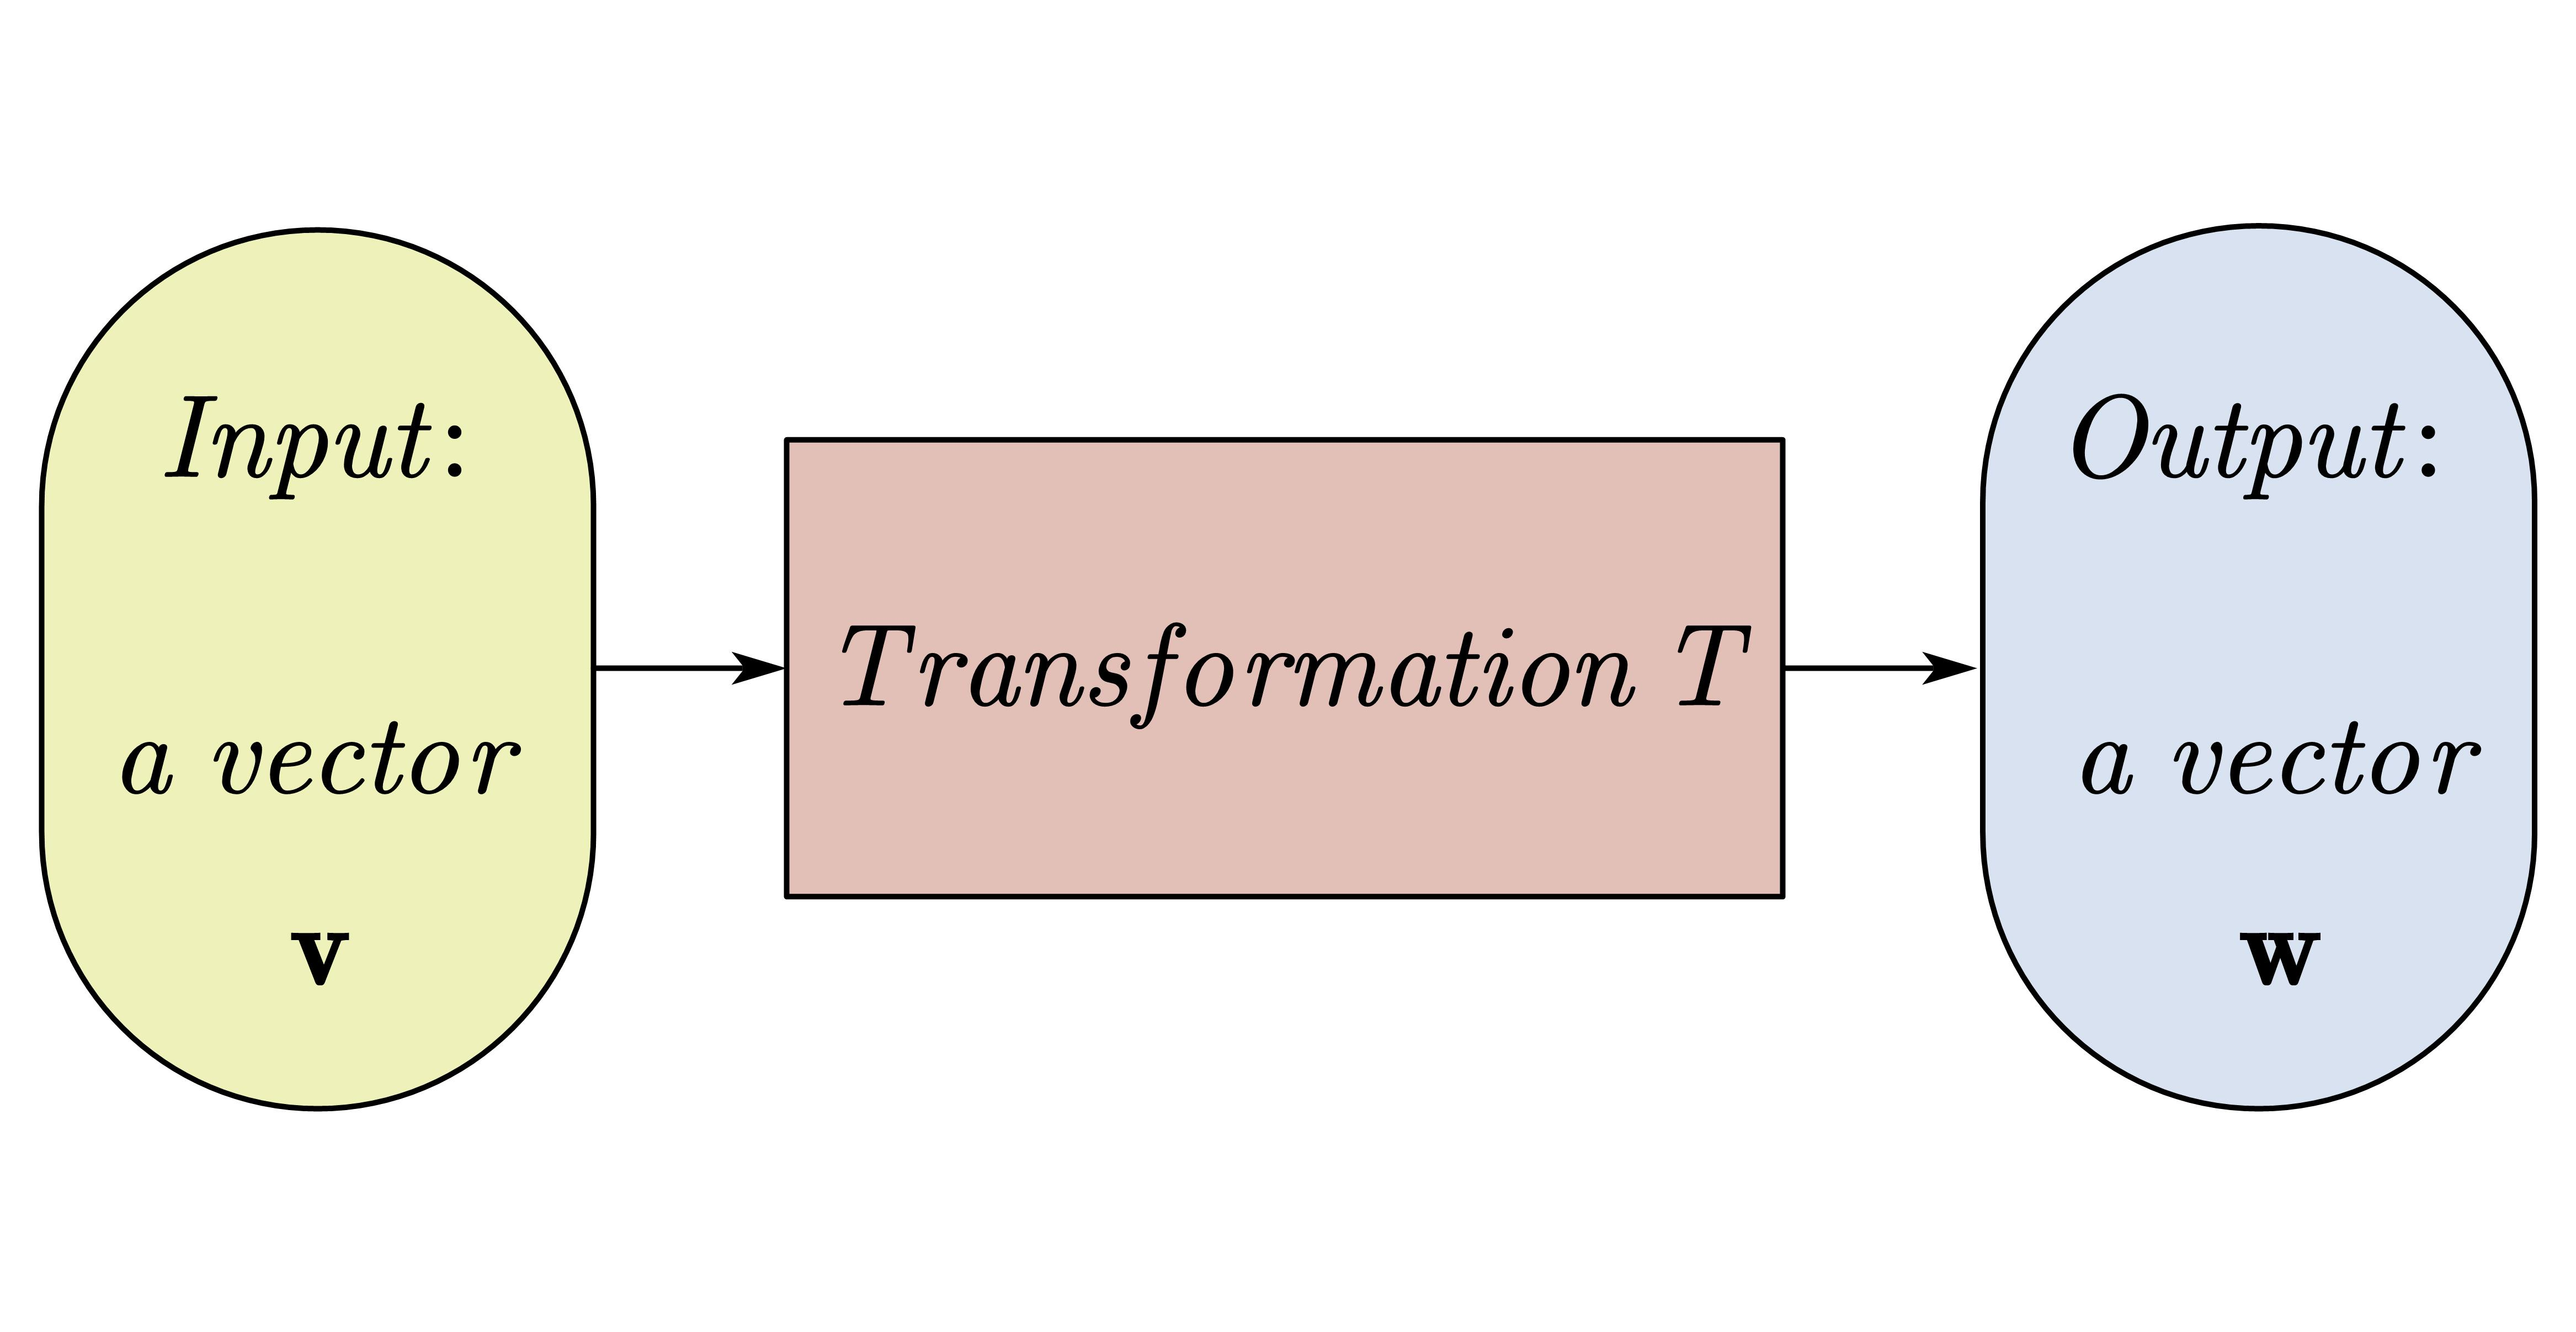
\includegraphics[width=0.52\textwidth]{transformation.jpg}
\end{figure}
\end{frame}

\begin{frame}{Linear Transfomations}
How to determine whether a transformation is linear?

\vspace{5pt}
Two rules:
\begin{itemize}
    \item Origin remains unchanged.
    \item Straight lines are still straight lines.
\end{itemize}

Generalize it and express in mathematical languages, a mapping $T$ is a linear transformation if
\begin{enumerate}
    \item $T\left( \mathbf{u}+\mathbf{v} \right) =T\left( \mathbf{u} \right) +T\left( \mathbf{v} \right)$
    \item $T\left( \alpha \mathbf{v} \right) =\alpha T\left( \mathbf{v} \right) $
\end{enumerate}
\begin{figure}
    \centering
    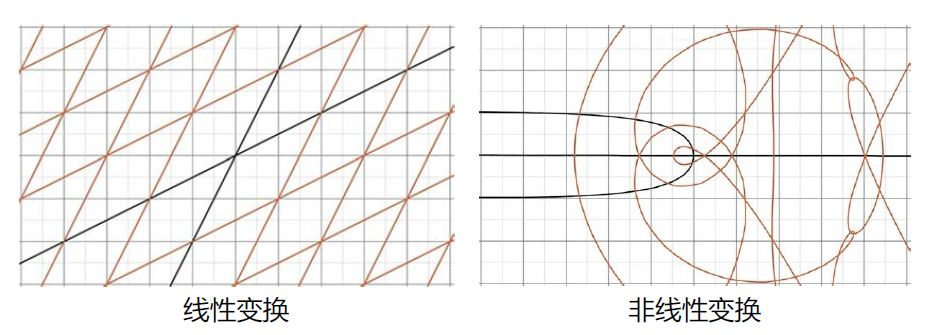
\includegraphics[width=0.7\textwidth]{lt.jpeg}
\end{figure}
\end{frame}

\begin{frame}{Matrix as Linear Transformation}
See this example of Linear Transformation:

\begin{figure}
    \centering
    \animategraphics[width=0.65\textwidth,loop,autoplay]{12}{./LinearT/LinearT_}{0}{79}
\end{figure}

To fully express a Linear Transformation, we can track the movement of two random vectors. Since we know that every vector in $\mathbb{R}^2$ space can be expressed by these 2 vectors!
\end{frame}

\begin{frame}{Matrix as Linear Transformation}
\begin{figure}
    \centering
    \animategraphics[width=0.4\textwidth,loop,autoplay]{12}{./LinearT/LinearT_}{0}{79}
\end{figure}
\vspace{-3pt}
Track the two unit vectors (the red one and the green one).
\vspace{3pt}
\begin{columns}
\column{0.5\textwidth}
\hspace{5pt}Before transformation:
\vspace{-3pt}
\begin{equation*}
    \boldsymbol{\hat{i}}=\left[ \begin{array}{c}
	1\\
	0\\
\end{array} \right] ,  \boldsymbol{\hat{j}}=\left[ \begin{array}{c}
	0\\
	1\\
\end{array} \right]
\end{equation*}

\column{0.5\textwidth}
\hspace{5pt}After transformation:\
\vspace{-3pt}
\begin{equation*}
    T(\boldsymbol{\hat{i}})=\left[ \begin{array}{c}
	2\\
	1\\
\end{array} \right] ,  T(\boldsymbol{\hat{j}})=\left[ \begin{array}{c}
	0\\
	1\\
\end{array} \right]
\end{equation*}
\end{columns}
\vspace{3pt}
Then the linear transformation can be expressed by a matrix:
    \begin{equation*}
        A= \left[ \begin{matrix}
    	2&		0\\
    	1&		1\\
    \end{matrix} \right] ,
    \end{equation*}

where the first column is the vector $\boldsymbol{\hat{i}}$ after transformation, the second column is the vector $\boldsymbol{\hat{j}}$ after transformation.
\end{frame}

\begin{frame}{Matrix as Linear Transformation}
Why we trace the movement of the unit vectors? Reasons?

\vspace{3pt}
Recall the definitions of linear transformations.

\vspace{3pt}
\begin{enumerate}
    \item $T\left( \mathbf{u}+\mathbf{v} \right) =T\left( \mathbf{u} \right) +T\left( \mathbf{v} \right)$
    \item $T\left( \alpha \mathbf{v} \right) =\alpha T\left( \mathbf{v} \right) $
\end{enumerate}

\vspace{-3pt}
Suppose we have an input vector $\left[ \begin{array}{c}
	x\\
	y\\
\end{array} \right]=x\left[ \begin{array}{c}
	1\\
	0\\
\end{array} \right]+y\left[ \begin{array}{c}
	0\\
	1\\
\end{array} \right]$, the vector after transformation is $T\left(\left[ \begin{array}{c}
	x\\
	y\\
\end{array}\right]\right)=xT\left(\left[ \begin{array}{c}
	1\\
	0\\
\end{array}\right]\right)+yT\left(\left[ \begin{array}{c}
	0\\
	1\\
\end{array} \right]\right)$.

\begin{equation*}
T\left(\left[ \begin{array}{c}
	x\\
	y\\
\end{array}\right]\right)=x\left[ \begin{array}{c}
	2\\
	1\\
\end{array}\right]+y\left[ \begin{array}{c}
	0\\
	1\\
\end{array} \right]=\left[ \begin{matrix}
	2&		0\\
	1&		1\\
\end{matrix} \right] \left[ \begin{array}{c}
	x\\
	y\\
\end{array} \right]
\end{equation*}
\vspace{5pt}
\begin{equation*}
    \left[ \begin{array}{c}
        x_{in}\\
        y_{in}\\
    \end{array} \right] \xrightarrow[Transformation\,\,Matrix\,\,\boldsymbol{A}]{Linear\,\,Transformation\,\,\boldsymbol{T}}\left[ \begin{array}{c}
        x_{out}\\
        y_{out}\\
    \end{array} \right]
\end{equation*}

\end{frame}

\begin{frame}{A Summary by Now}
    \begin{figure}
        \centering
        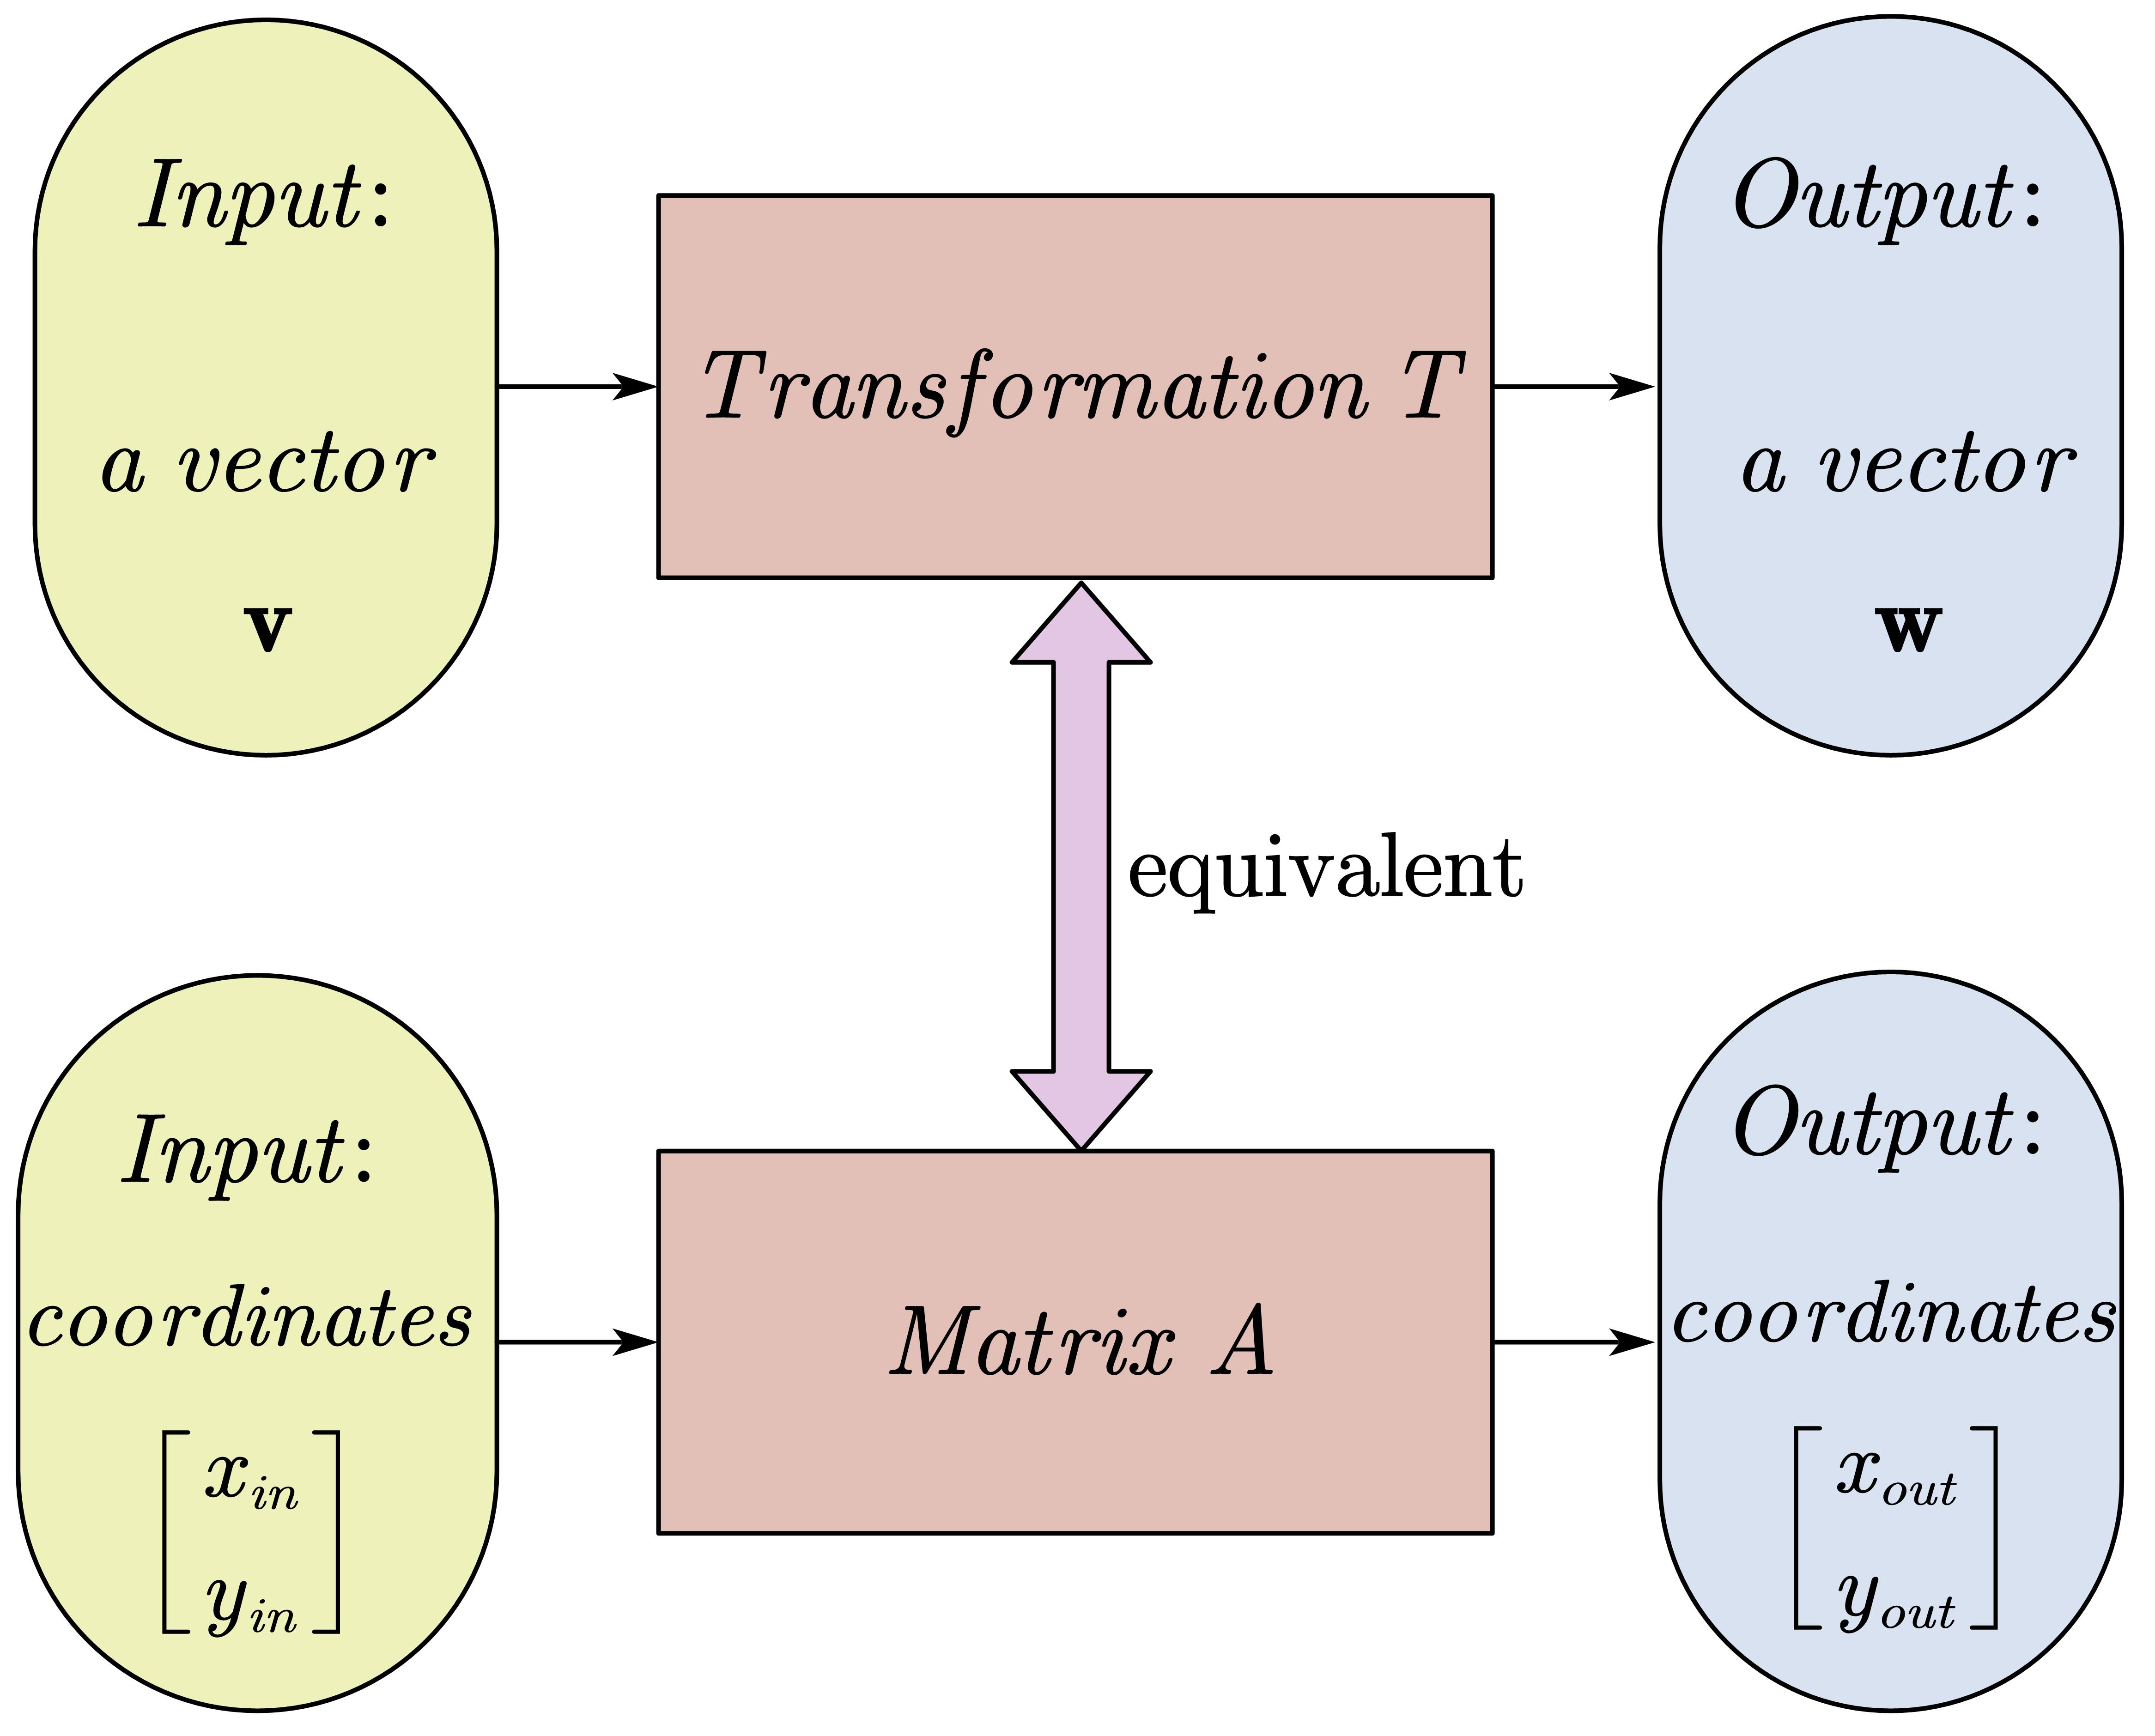
\includegraphics[width=0.7\textwidth]{transformation2.jpg}
    \end{figure}

    \begin{center}
        Video: \url{https://www.bilibili.com/video/BV1ys411472E?p=4}
    \end{center}

\end{frame}

\begin{frame}{A New Perspective: Understanding Matrices}
Now, every time you meet a matrix, try to see it as a linear transformation, imagine the transformation in your mind.

\begin{enumerate}
    \item Identity matrix: $\left[ \begin{matrix}
        1&		0\\
        0&		1\\
    \end{matrix} \right]$, do nothing.
    \item Permutation matrix: $\left[ \begin{matrix}
        0&		1\\
        1&		0\\
    \end{matrix} \right]$, exchange axis.
    \item Rotation matrix: $\left[ \begin{matrix}
        0&		-1\\
        1&		0\\
    \end{matrix} \right]$, rotate the plane by 90$^\circ$ anti-clockwise.
    \item Reflection matrix: $\left[ \begin{matrix}
        1&		0\\
        0&		-1\\
    \end{matrix} \right]$, reflection by $x$ axis.
    \item Projection matrix: $\left[ \begin{matrix}
        1&		0\\
        0&		0\\
    \end{matrix} \right]$, projection on $x$ axis.
\end{enumerate}
Give me a matrix that can rotate the plane by 30$\circ$ clockwise.
\end{frame}

\begin{frame}{A New Perspective: Understanding Matrix Multiplication}
I have once introduced you the column method of matrix multiplication without explanation, now give me a explanation from the linear transformation perspective.
\begin{equation*}
    \left[ \begin{matrix}
        1&		1\\
        0&		1\\
    \end{matrix} \right] \left[ \begin{array}{c}
        x\\
        y\\
    \end{array} \right] =x\left[ \begin{array}{c}
        1\\
        0\\
    \end{array} \right] +y\left[ \begin{array}{c}
        1\\
        1\\
    \end{array} \right] =\left[ \begin{array}{c}
        x+y\\
        y\\
    \end{array} \right]
\end{equation*}


If I multiply 2 matrices together (and they can be multiplied), what will we get? Still a matrix! That means it is still a linear transformation!

\begin{equation*}
    \left[ \begin{matrix}
        0&		-1\\
        1&		0\\
    \end{matrix} \right] \left[ \begin{matrix}
        0&		-1\\
        1&		0\\
    \end{matrix} \right] =\left[ \begin{matrix}
        -1&		0\\
        0&		-1\\
    \end{matrix} \right]
\end{equation*}

\vspace{3pt}
The matrix multiplication process is to find the total linear transformation.
\end{frame}

\begin{frame}{A New Perspective: Understanding Inverses}
Can I find an invert transformation, get the coordinates before transformation?

\vspace{3pt}
Rotation matrix: $\left[ \begin{matrix}
    0&		-1\\
    1&		0\\
\end{matrix} \right]$, rotate the whole plane by 90$^\circ$ anti-clockwise.

\vspace{3pt}
It is invertible. Show me the inverse of this rotation matrix (which is a matrix that can rotate the whole plane by 90$^\circ$ clockwise definitely).

\vspace{3pt}
A matrix: $\left[ \begin{matrix}
    1&		2\\
    3&		6\\
\end{matrix} \right]$.

\vspace{3pt}
We have seen this matrix before... It is not invertible. Try to explain that from the linear transformation perspective.

\vspace{3pt}
Many vectors result in a single vector, and I cannot find an invert transformation to transform an input vector to multiple output vectors.
\end{frame}

\begin{frame}{A New Perspective: Understanding Column Space; Rank}
A matrix: $\left[ \begin{matrix}
    1&		2\\
    3&		6\\
\end{matrix} \right]$, think about its column space and rank.

\vspace{3pt}
The column space is a straight line in $\mathbb{R}^2$ plane, which is also the space consists of all the possible output vectors. The rank is the dimension of the column space, which gives us a description about the dimension of output space.

\vspace{3pt}
How about the non-square matrices? Consider the following matrix $A$.
\begin{equation*}
    \left[ \begin{matrix}
        1&		2\\
        2&		1\\
        4&		3\\
    \end{matrix} \right]
\end{equation*}

The input is a vector in $\mathbb{R}^2$, output is a vector in $\mathbb{R}^3$. The 2 unit vectors $[1\:0]^T, [0\:1]^T$ are transformed to 2 vectors in $\mathbb{R}^3$. Imagine the linear transformation represented by matrix $A$, it transforms the $\mathbb{R}^2$ plane to a 2-dimensional plane in $\mathbb{R}^3$. The rank (2 in this example) gives us the dimension of the output space.
\end{frame}

\begin{frame}{A New Perspective: Understanding Solvability Condition}
A linear system $Ax=b$ is solvable if and only if $b$ is in column space of $A$.

\vspace{3pt}
The column space of $A$ is the whole output space of the linear transformation represented by $A$. If a vector $b$ is not in the column space, then we cannot have a solution because no input vectors will result in $b$ after linear transformation.

\vspace{3pt}
Example:
\begin{equation*}
    \left[ \begin{matrix}
        1&		2\\
        3&		6\\
    \end{matrix} \right] \left[ \begin{array}{c}
        x_1\\
        x_2\\
    \end{array} \right] =\left[ \begin{array}{c}
        1\\
        2\\
    \end{array} \right]
\end{equation*}
This linear system is definitely inconsistent because transform a vector to a line will not result in a vector not in that line.
\end{frame}

\begin{frame}
    \begin{figure}
        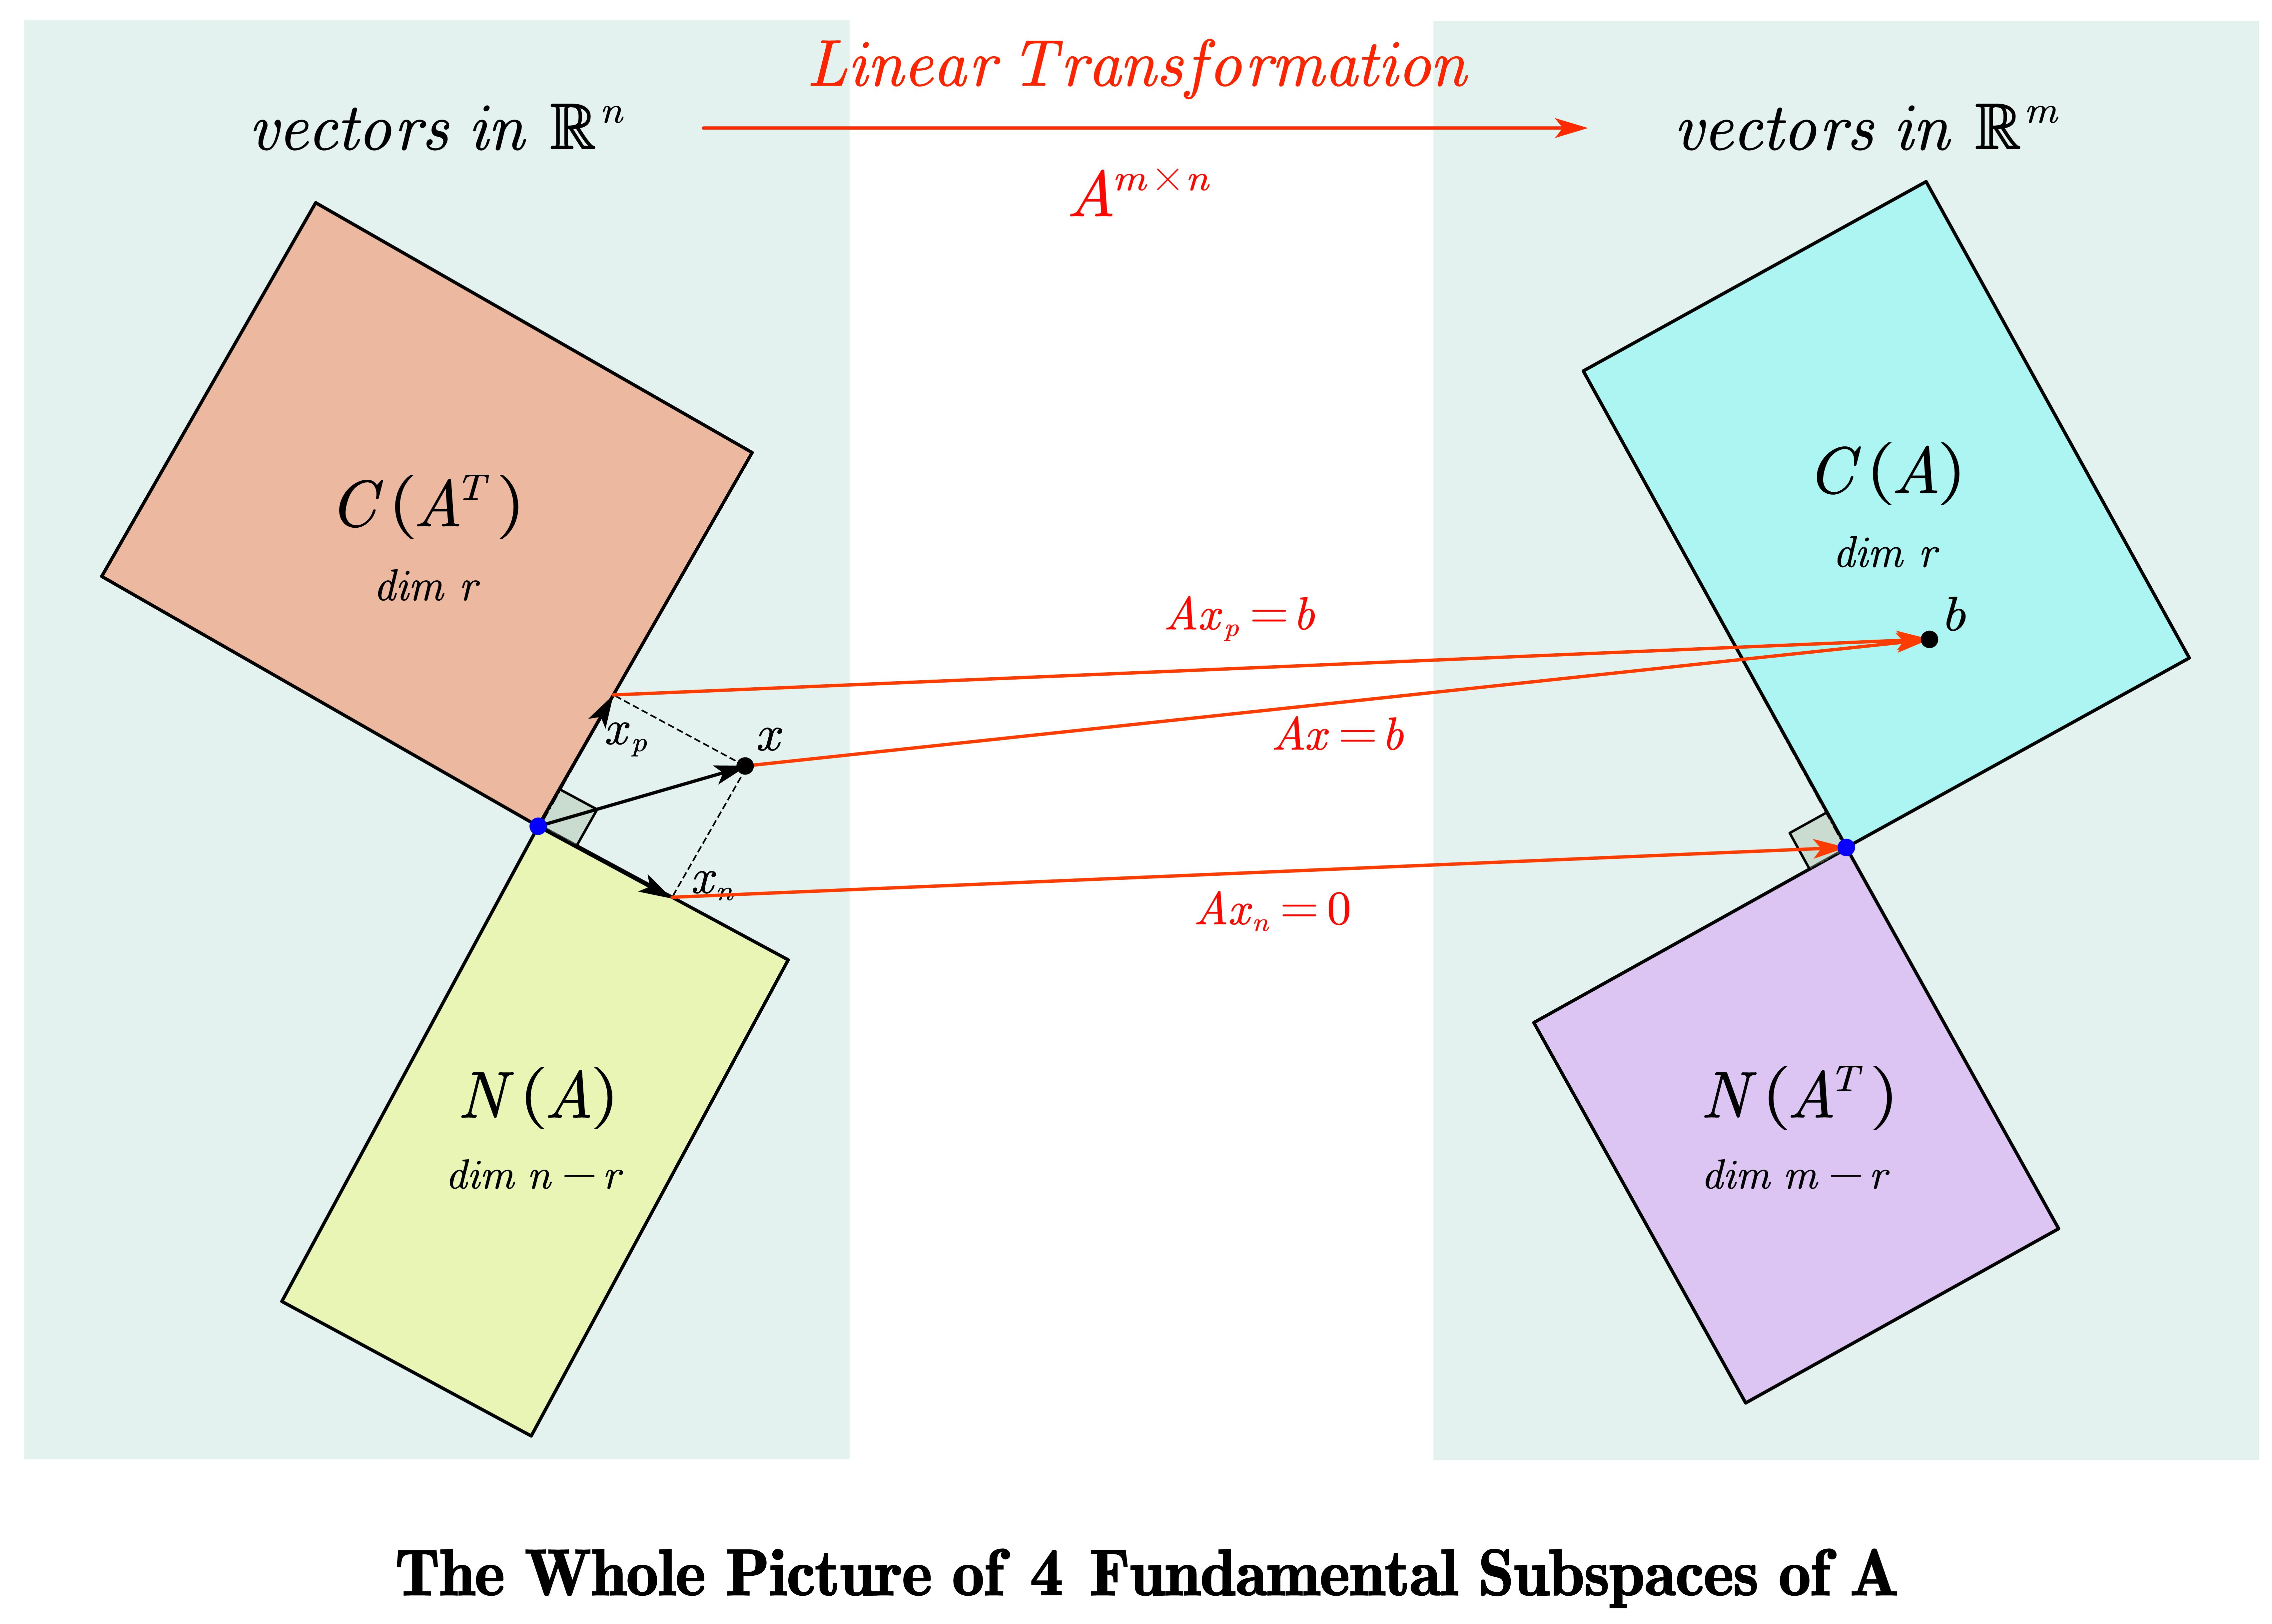
\includegraphics[width=0.96\textwidth]{WHOLE.jpg}
    \end{figure}
\end{frame}

\section{Transformation Matrix in Other Basis}
\begin{frame}{Coordinates and Basis}
In previous slides, we always represent vectors by coordinates such as $\left[ \begin{array}{c}
	1\\
	2\\
\end{array} \right]$, $\left[ \begin{array}{c}
	3\\
	2\\
    7\\
\end{array} \right]$. That is natural because we use the standard basis! For example:
\begin{equation*}
    \left[ \begin{array}{c}
        1\\
        2\\
    \end{array} \right] =1\left[ \begin{array}{c}
        1\\
        0\\
    \end{array} \right] +2\left[ \begin{array}{c}
        0\\
        1\\
    \end{array} \right]
\end{equation*}

\vspace{3pt}
But, a space can have infinite bases, if we change the basis, the coordinates will also change. Suppose we choose $\left[ \begin{array}{c}
    1\\
    1\\
\end{array} \right]$ and $\left[ \begin{array}{c}
    0\\
    1\\
\end{array} \right]$ as a basis, then the coordinates becomes $\left[ \begin{array}{c}
    1\\
    1\\
\end{array} \right]$ because:
\begin{equation*}
    \left[ \begin{array}{c}
        1\\
        2\\
    \end{array} \right] =1\left[ \begin{array}{c}
        1\\
        1\\
    \end{array} \right] +1\left[ \begin{array}{c}
        0\\
        1\\
    \end{array} \right]
\end{equation*}

A summary: coordinates come from the choice of basis.
\end{frame}

\begin{frame}{The Transformation Matrix with Other Basis}
Our transformation matrix $A$ do the easy thing: input the coordinates before transformation, and output the coordinates after transformation.

Let's now consider the new basis for $\mathbb{R}^2$: $\left[ \begin{array}{c}
    1\\
    1\\
\end{array} \right]$ and $\left[ \begin{array}{c}
    0\\
    1\\
\end{array} \right]$.

Suppose an input coordinates $\left[ \begin{array}{c}
	x\\
	y\\
\end{array} \right]\left(x\left[ \begin{array}{c}
	1\\
	1\\
\end{array} \right]+y\left[ \begin{array}{c}
	0\\
	1\\
\end{array} \right]\right)$, the coordinates after transformation is $T\left(\left[ \begin{array}{c}
	x\\
	y\\
\end{array}\right]\right)=xT\left(\left[ \begin{array}{c}
	1\\
	1\\
\end{array}\right]\right)+yT\left(\left[ \begin{array}{c}
	0\\
	1\\
\end{array} \right]\right)$.

\begin{equation*}
    T\left( \left[ \begin{array}{c}
        x\\
        y\\
    \end{array} \right] \right) =\left[ \begin{matrix}
        &		\\
        T\left( \left[ \begin{array}{c}
        1\\
        1\\
    \end{array} \right] \right)&		T\left( \left[ \begin{array}{c}
        0\\
        1\\
    \end{array} \right] \right)\\
        &		\\
    \end{matrix} \right] \left[ \begin{array}{c}
        x\\
        y\\
    \end{array} \right]
\end{equation*}

Things get easier now. Every column in transformation matrix $A$ is the output coordinates of an input basis vector.
\end{frame}

\begin{frame}{Example}
\begin{example}
Let $L$: $\mathbb{R}^2\rightarrow \mathbb{R}^3$ be the linear transformation defined by
\begin{equation*}
    L\left( \mathbf{x} \right) =\left[ \begin{array}{c}
        x_2\\
        x_1+x_2\\
        x_1-x_2\\
    \end{array} \right]
\end{equation*}
Find the matrix representations of $L$ with respect to the ordered bases $\left\{ \mathbf{u}_{\mathbf{1}},\mathbf{u}_{\mathbf{2}} \right\}$ and $\left\{ \mathbf{b}_{\mathbf{1}},\mathbf{b}_{\mathbf{2}},\mathbf{b}_{\mathbf{3}} \right\}$, where
\begin{equation*}
    \mathbf{u}_{\mathbf{1}}=\left[ \begin{array}{c}
        1\\
        2\\
    \end{array} \right] , \mathbf{u}_2=\left[ \begin{array}{c}
        3\\
        1\\
    \end{array} \right]
\end{equation*}
\vspace{-2pt}
and
\vspace{-2pt}
\begin{equation*}
    \mathbf{b}_{\mathbf{1}}=\left[ \begin{array}{c}
        1\\
        0\\
        0\\
    \end{array} \right] , \mathbf{b}_2=\left[ \begin{array}{c}
        1\\
        1\\
        0\\
    \end{array} \right], \mathbf{b}_3=\left[ \begin{array}{c}
        1\\
        1\\
        1\\
    \end{array} \right]
\end{equation*}
\end{example}
\end{frame}

\begin{frame}{Example}
\textbf{Solution:}\newline
Input coordinates $\left[ \begin{array}{c}
    1\\
    0\\
\end{array} \right]$, which is $\left[ \begin{array}{c}
    1\\
    2\\
\end{array} \right]$ in natural basis.

The output in natural basis will be
\begin{equation*}
    L\left( \left[ \begin{array}{c}
        1\\
        2\\
    \end{array} \right] \right) =\left[ \begin{array}{c}
        2\\
        1+2\\
        1-2\\
    \end{array} \right] =\left[ \begin{array}{c}
        2\\
        3\\
        -1\\
    \end{array} \right]
\end{equation*}
Transform to the coordinates under new basis $\mathbf{b}$.
\begin{equation*}
    \left[ \begin{array}{c}
        2\\
        3\\
        -1\\
    \end{array} \right] =a_{11}\left[ \begin{array}{c}
        1\\
        0\\
        0\\
    \end{array} \right] +a_{21}\left[ \begin{array}{c}
        1\\
        1\\
        0\\
    \end{array} \right] +a_{31}\left[ \begin{array}{c}
        1\\
        1\\
        1\\
    \end{array} \right]
\end{equation*}
Output coordinates $\left[ \begin{array}{c}
    -1\\
    4\\
    -1\\
\end{array} \right]$, which is $\left[ \begin{array}{c}
    2\\
    3\\
    -1\\
\end{array} \right]$ in natural basis.
\end{frame}

\begin{frame}{Example}
\textbf{Solution:}\newline
Input coordinates $\left[ \begin{array}{c}
    0\\
    1\\
\end{array} \right]$, which is $\left[ \begin{array}{c}
    3\\
    1\\
\end{array} \right]$ in natural basis.

The output in natural basis will be
\begin{equation*}
    L\left( \left[ \begin{array}{c}
        3\\
        1\\
    \end{array} \right] \right) =\left[ \begin{array}{c}
        1\\
        3+1\\
        3-1\\
    \end{array} \right] =\left[ \begin{array}{c}
        1\\
        4\\
        2\\
    \end{array} \right]
\end{equation*}
Transform to the coordinates under new basis $\mathbf{b}$.
\begin{equation*}
    \left[ \begin{array}{c}
        1\\
        4\\
        2\\
    \end{array} \right] =a_{12}\left[ \begin{array}{c}
        1\\
        0\\
        0\\
    \end{array} \right] +a_{22}\left[ \begin{array}{c}
        1\\
        1\\
        0\\
    \end{array} \right] +a_{32}\left[ \begin{array}{c}
        1\\
        1\\
        1\\
    \end{array} \right]
\end{equation*}
Output coordinates $\left[ \begin{array}{c}
    -3\\
    2\\
    2\\
\end{array} \right]$, which is $\left[ \begin{array}{c}
    1\\
    4\\
    2\\
\end{array} \right]$ in natural basis.
\end{frame}
\end{document}